\section{Analysis of Memcached attack phases}
\label{sec4}

Due to the size and scope of the \gls{sanren} network, the \gls{sanren} \gls{csirt} is notified of multiple attacks on a regular basis. This attack analysis will focus specifically on the Memcached attack and how the attack was  observed and mitigated within the \gls{sanren} environment.



\textit{Figure~\ref{fig:time_line}} depicts the time-line of the Memcached attack. On 22 February 2018, the US-\gls{cert} sent out an alert sating that the Memcached protocol is vulnerable to \gls{drdos} attacks   \cite{USCert2018}. According to \cite{Akamai2018Memcached}, the attack reached its peek on 28 February 2018. According to \cite{DDoSMon}, a \gls{ddos} monitoring company, the Memcached attacks started drastically decreasing in size from 6 March 2018.

\begin{figure}[h]
    \centering
    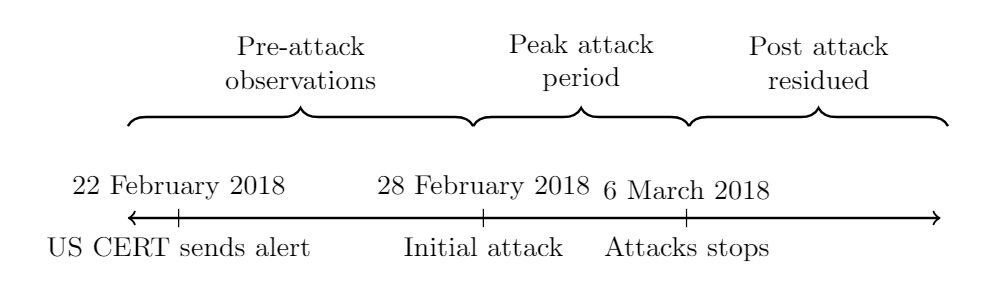
\includegraphics[width=\columnwidth]{section_4/memcached_phases.JPG}
    \caption{Memcached attack time-line}
    \label{fig:time_line}
\end{figure}

In the remainder of this sub-section the various phases of the attack will be analysed using the network flow data obtained from the \gls{sanren} NetFlow collector.

\subsection{Pre-attack observations}
\label{sub-pre-attack}

Once the security alert was posted by the US-\gls{cert}, the \gls{sanren} \gls{csirt} modified the network flow analysis system to notify the CSIRT if any anomalies are detected on port 11 211, the default Memcached service port. The CSIRT also identified all active Memcached servers on the \gls{sanren} network using the NetFlow data set. Prior to the initial attack only four Memcached servers were detected.



Prior to the Memcached attack disclosure, the \gls{sanren} network observed approximately 2.8 Megabytes of data, resulting from 917 flows per day\footnote{Average data rate observed for period 1 January 2018 -- 10 February 2018}. In \textit{Figures~\ref{fig:pre_graph_bytes}--~\ref{fig:pre_graph_bpf}}, three graphs are presented representing the Memcached traffic observed prior to the primary attack date. The first graph depicts the traffic in bytes observed during this period, the second graph plots the number of flows observed and the third graph plots the \gls{bpf} for the period.

\begin{figure}
    \centering
    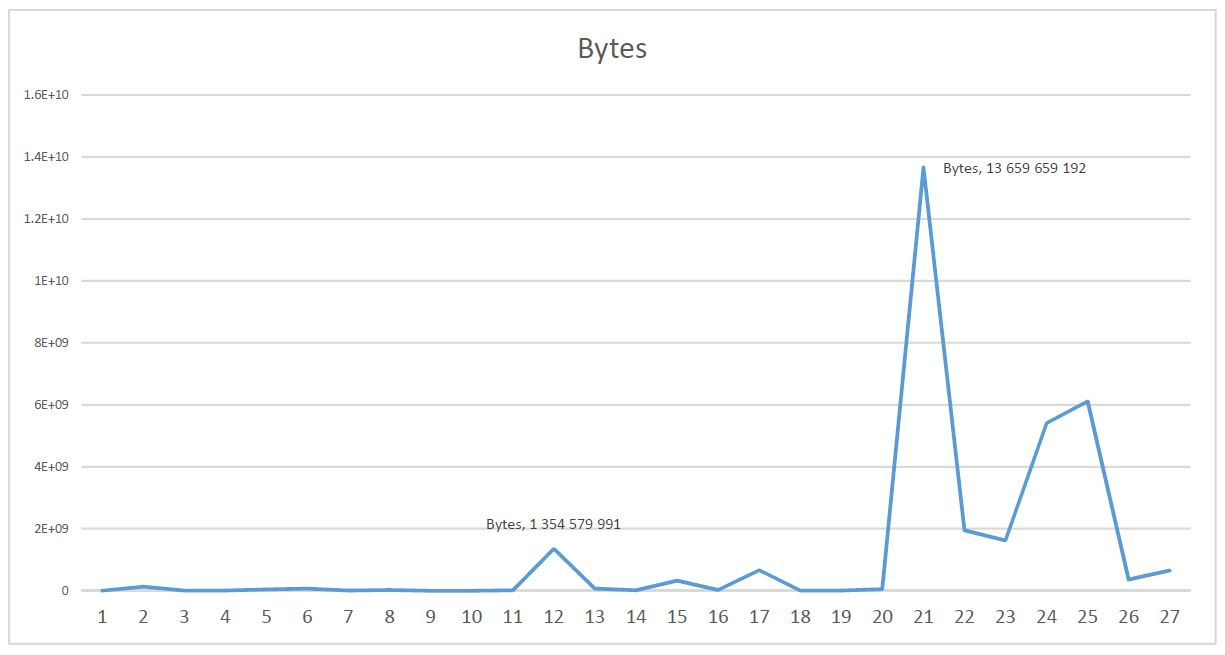
\includegraphics[width=\columnwidth]{section_4/memcached_pre-attack_bytes.JPG}
    \caption{Pre-attack Memcached protocol activity bytes observed}
    \label{fig:pre_graph_bytes}
\end{figure}

\begin{figure}
    \centering
    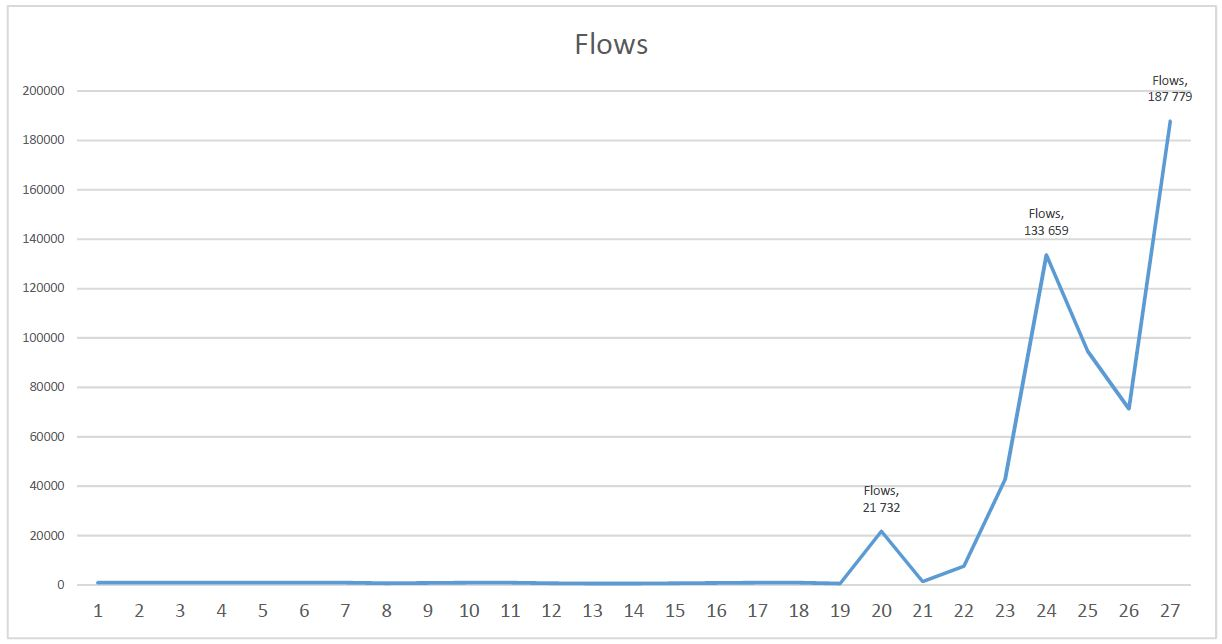
\includegraphics[width=\columnwidth]{section_4/memcached_pre-attack_flows.JPG}
    \caption{Pre-attack Memcached protocol activity flows observed }
    \label{fig:pre_graph_flows}
\end{figure}

\begin{figure}
    \centering
    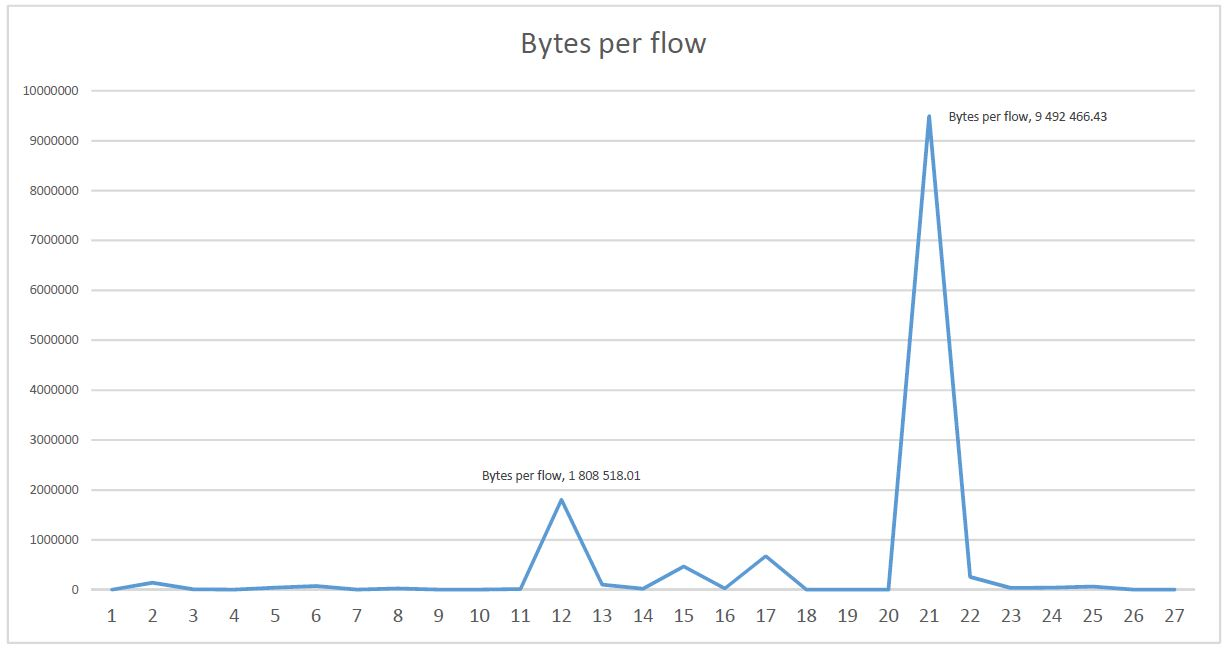
\includegraphics[width=\columnwidth]{section_4/memcached_pre-attack_bpf.JPG}
    \caption{Pre-attack Memcached protocol activity bytes per flow observed }
    \label{fig:pre_graph_bpf}
\end{figure}
In the first graph, \textit{Figure~\ref{fig:pre_graph_bytes}}, a large spike in network traffic is observed (13 Gigabyte in one day) on 21 February 2018, the day before the US-\gls{cert} sent out the advisory. A smaller increase in bandwidth usage can also be observed on 12 February 2018 (1.3 Gigabyte of data). 



In the second graph, \textit{Figure~\ref{fig:pre_graph_flows}}, it is shown that the number of flows associated with the Memcached service greatly increased since 23 February. Despite the increase in the number of flows, the data usage did not increase at a similar rate, to that of the flow count. The number of flows per day increase by 20 000 \%, from an average of 939 to a maximum of 187 779. Unlike in graph one, the number of flows did not have a notable increase on 12 February. 



In the third graph, \textit{Figure~\ref{fig:pre_graph_bpf}}, there is a noticeable increase in \gls{bpf} observed on 21 February 2018. A sudden increase in \gls{bpf} is an indicator for amplification. The \gls{bpf} graph indicates that amplification traffic was observed before the US-\gls{cert} sent out the alert. On average the Memcached service produced a 30 Kilobyte response per flow, prior to the vulnerability disclosure. On 21 February, 9.5 Megabyte of data was generated per flow.  

Based on the NetFlow sensor analysis the majority of the flows observed between 23 February 2018 and 27 February 2018, were as a result of port scans and service discovery scans. These flows represent 93.7 \% of all flows observed in this period. The observed service discovery flows exhibit the following properties:
\begin{itemize}
    \item Destination port 11 211 (Memcached),
    \item \gls{udp} protocol,
    \item Memcached request flow, payload size  \textless 49 bytes.
    \item Memcached response flow, payload size  \textless 107 bytes.
    \item Source IP distribution:   185.176.192.244 (40.6\%),  185.94.111.1 (21.5\%),\newline  185.194.112.10 (16.5\%) and other (21.4\%)\footnote{Due to IP spoofing, the source IP detected by the network flow sensor may be inaccurate \cite{senie1998network}.}.
\end{itemize}

\subsection{Peak attack period}
\label{sub-during-attack}

According to \cite{Akamai2018Memcached}, the primary Memcached attack period was between 28 February 2018 and 6 March 2018. During the peak traffic period, five Memcached servers were observed.

According to \cite{Shodan}, a search engine for vulnerable Internet-connected devices, there were 87 811 Internet facing Memcached servers worldwide on 28 March 2018. Of all the servers observed, only 212 of these servers were located within South Africa and only 4 were hosted by \gls{sanren}.


At 8 AM SAST, 1 March 2018, the \gls{sanren} \gls{csirt} were notified of the sudden increase in Memcached activity and by 9H30 AM SAST, 1 March 2018, the four servers which were observed during the pre-attack phase were patched. Memcached request messages were still received by the servers, but no Memcached responses were issued to servers outside the local network IP address ranges. On 2 March 2018 a fifth Memcached server became active on the \gls{sanren} network. Due to the servers limited bandwidth it produced significantly less traffic than the initial four servers.  

\textit{Table~\ref{tab:memcached_sum}} summarises the average data flow activity observed by the \gls{sanren} network flow collector for this period. The server IP addresses and host names have been anonymised to protect the \gls{sanren} users.

% \begin{figure}
%     \centering
%     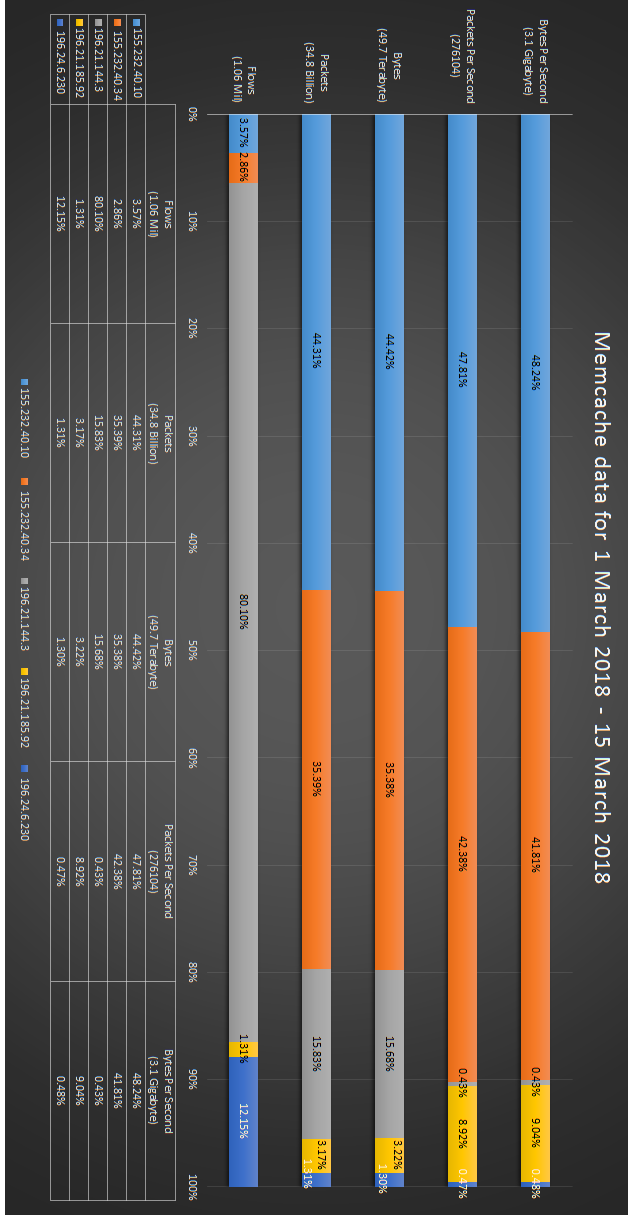
\includegraphics[width=\columnwidth]{section_4/Memcached_march_2018.png}
%     \caption{Memcached data for March 2018}
%     \label{fig:4memcached}
% \end{figure}


\begin{table}[h]
\caption{Summary of \gls{ddos} activity observed during peak attack period}
\label{tab:memcached_sum}
\begin{tabular}{l|r|r|r|r|r|}
\cline{2-6}
                              & \multicolumn{1}{l|}{Flows} & \multicolumn{1}{l|}{Packets} & \multicolumn{1}{l|}{Bytes} & \multicolumn{1}{l|}{\begin{tabular}[c]{@{}l@{}}Packets \\ /second\end{tabular}} & \multicolumn{1}{l|}{\begin{tabular}[c]{@{}l@{}}Bytes \\ /second\end{tabular}} \\ \hline
\multicolumn{1}{|l|}{Server 1} & $38 076$                   & $1.54e+10$                   & $2.12e+13$                 & $132 005$                                                                       & $1.5e+9$                                                                      \\ \hline
\multicolumn{1}{|l|}{Server 2} & $30 470$                   & $1.23e+10$                   & $1.76e+13$                 & $117 001$                                                                       & $1.3e+9$                                                                      \\ \hline
\multicolumn{1}{|l|}{Server 3} & $853 755$                  & $5.5e+9$                     & $7.8e+12$                  & $1 177$                                                                         & $1.33e+7$                                                                     \\ \hline
\multicolumn{1}{|l|}{Server 4} & $13 970$                   & $1.1e+9$                     & $1.6e+12$                  & $24 616$                                                                        & $2.81e+8$                                                                    \\ \hline
\multicolumn{1}{|l|}{Server 5} & $129 528$                  & $4.55e+8$                    & $1.6e+12$                  & $1 305$                                                                         & $1.49e+7$                                                                     \\ \hline
\multicolumn{1}{|l|}{Total}    & $1.06e+6$                  & $3.48e+10$                   & $4.97e+13$                 & 276 104                                                                         & $3.1e+9$                                                                      \\ \hline
\end{tabular}
\end{table}

% \begin{table*}[]
% \caption{Summary of \gls{ddos} activity observed during peak attack period}
% \label{tab:memcached_sum}
% \begin{tabular}{l|r|r|r|r|r|}
% \cline{2-6}
%                               & \multicolumn{1}{l|}{Flows} & \multicolumn{1}{l|}{Packets} & \multicolumn{1}{l|}{Bytes} & \multicolumn{1}{l|}{\begin{tabular}[c]{@{}l@{}}Packets \\ /second\end{tabular}} & \multicolumn{1}{l|}{\begin{tabular}[c]{@{}l@{}}Bytes \\ /second\end{tabular}} \\ \hline
% \multicolumn{1}{|l|}{Server 1} & \num{38 076}                   & \num{1.54e+10}                   & \num{2.12e+13}                 & \num{132 005}                                                                       & \num{1.5e+9}                                                                      \\ \hline
% \multicolumn{1}{|l|}{Server 2} & \num{30 470}                   & \num{1.23e+10}                   & \num{1.76e+13}                 & \num{117 001}                                                                       & \num{1.3e+9}                                                                      \\ \hline
% \multicolumn{1}{|l|}{Server 3} & \num{853 755}                  & \num{5.5e+9}                     & \num{7.8e+12}                  & \num{1 177}                                                                         & \num{1.33e+7}                                                                     \\ \hline
% \multicolumn{1}{|l|}{Server 4} & \num{13 970}                   & \num{1.1e+9}                     & \num{1.6e+12}                  & \num{24 616}                                                                        & \num{2.81e+8}                                                                    \\ \hline
% \multicolumn{1}{|l|}{Server 5} & \num{129 528}                  & \num{4.55e+8}                    & \num{1.6e+12}                  & \num{1 305}                                                                         & \num{1.49e+7}                                                                     \\ \hline
% \multicolumn{1}{|l|}{Total}    & \num{1.06e+6}                  & \num{3.48e+10}                   & \num{4.97e+13}                 & \num{276 104}                                                                         & \num{3.1e+9}                                                                      \\ \hline
% \end{tabular}
% \end{table*}





Over the 6 day period 49.7 Terabytes of data was generated by the Memcached servers of which 48.6 Terabytes were transmitted between 10 PM SAST, 28 February 2018 and 10 AM SAST, 1 March 2018. At its peek, Server 1 and Server 2 each produced 10.9 Gigabytes of traffic per second. The Memcached attack completely saturated the bandwidth allocated to Server 1 and Server 2. Server 1 and Server 2 only contributed to 6.43\% of the data flows observed during this period, but they contributed to 79.8\% of the traffic generated. On average, each flow generated by Server 1 and Server 2 produced 46.8 Megabytes of traffic. This is a significant increase from the 30 Kilobyte responses observed during the pre-attack observations. The average amplification factor observed by these servers were 1:49500.

Server 3 only had a one Megabyte connection with a four Megabyte Memcached cache. Due to Server 3's limited resources it produced significantly less response traffic than Server 1 and Server 2 despite receiving 80.1\% of the observed Memcached request flows. Server 4 had a 24 Megabyte bandwidth with a 64 Kilobyte Memcached cache. Though Server 4 had more bandwidth capacity than Server 3, it produced far less traffic than $Server 3$ due to the small cache size. The amplification factor of Server 4 was also the lowest of all observed servers due to the reduced cache size, only 1:1600. 

The \gls{sanren} \gls{csirt} applied software patches to Server 1 to 4 on 1 March 2018 at 10 AM SAST. Since the patches were applied, the servers still receive periodic service discovery probes and Memcached requests but they no longer respond to unverified requests.

Server 5's Memcached service only became active on 2 March 2018. Server 5 only had a one Megabyte international connection and a 128 Kilobyte Memcached cache. The server operator was not aware of the Memcached service being enabled on their server. The server only generated traffic directed at seven target IP addresses. According to the network flow data, Server 5 was also the victim of a brute force \gls{ssh} attack prior to the Memcached service starting up. Server 5 was not managed by the \gls{sanren} network operators, but by a private University systems administrator. Given the suspicious behaviour observed on Server 5, the \gls{sanren} \gls{csirt} notified the system administrator of the server and provided them with an analysis of the server's behaviour. 


An increase in the number of Memcached severs also increased world wide after the peek periods of attack. On 28 February, there were 214 South African and 87 811 international servers vulnerable to Memcached amplification, according to \cite{Shodan}. On 4 March 2018, the number of vulnerable servers in South Africa reached its peek, 236. At least 8 of the newly discovered South African servers were confirmed to be Honey Pots. The international vulnerable server count reached its peek on 7 March 2018, with 107 431 according to SHODAN's reporting tools  \citep{Shodan}. The international server count increased by 22.3\% during the attack period, thus far no information has been released as to how many of these server are Honey Pots.    

\cite{CyberReason},  discovered that attackers were embedding ransomware notes into the Memcached payloads. Figure.~\ref{fig:ransom} illustrates a sample payload. In the payload message the attacker requests the victim to pay 50 Monero, a crypto currency, into a crypto wallet account. According to Kerb \cite{kerbs2018Powerful} it is not clear if any victim's paid the ransom amount. The US-CERT and Cyber Reason warned victims not to pay the ransom since there was no guarantee that attacks would stop after the payment was made \citep{kerbs2018Powerful,CyberReason}.

\begin{figure}[H]
    \centering
    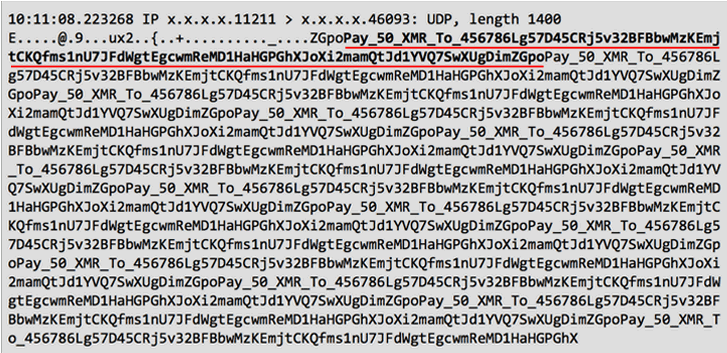
\includegraphics[width=\columnwidth]{section_4/ransom_memcached.PNG}
    \caption{Sample ransomware message in Memcached payload}
    \label{fig:ransom}
\end{figure}


\subsection{Post attack residue}
\label{sub-post-attack}


During the attack period 12 139 unique IP addresses were observed to be communicating over port 11 211 using the Memcached protocol on the \gls{sanren} network. As part of the post attack analysis, the network flow data was used to filter potential attack IP addresses from the victim IP addresses\footnote{It should be noted that,  IP addresses can be spoofed when using \gls{udp} traffic \cite{senie1998network}.}.  As part of our classification several metrics were defined to either include or exclude a candidate IP address as an attacker or victim. These criteria are as follows:
\begin{itemize}
    \item If the IP address belongs to a known legitimate user of Memcached service, label the IP as $benign$. 
    \item If the number of Memcached requests issued per day increased by more than 50\% after 21 February, the IP was labelled as $suspicious$.
    \item If the ratio of request traffic to response traffic generated by the IP was greater than 1:100, the IP was labelled as a $victim$.
    \item If any of the other network flow sensors\footnote{The sensor to detect port scanning activity is based on the \gls{taps} algorithm, proposed by \cite{sridharan2006connectionless}. \gls{taps} port scan detection technique will be discussed in greater detail in sub-section \ref{sec4_port_scan}.}, deployed by the \gls{sanren} \gls{csirt}, detected the IP as a port scanner, the IP was labelled as a $port\_scanner$. 
    \item If any of the the $port\_scanner$ IP addresses were found to only be scanning for port 11 211 and using the Memcached protocol, it was assigned an additional label, $memcached\_scanner$. 
\end{itemize}
\textit{Table~\ref{tab:IP_sum}} summarises labels assigned to IP addresses during each phase.

\begin{table}[h]
\caption{Summary of IP addresses observed during Memcached attack}
\label{tab:IP_sum}
\begin{tabular}{l|r|r|r|r|r|}
\cline{2-6}
                                                                             & \multicolumn{1}{l|}{Observed} & \multicolumn{1}{l|}{Benign} & \multicolumn{1}{l|}{\begin{tabular}[c]{@{}l@{}}Port\\ Scanner\end{tabular}} & \multicolumn{1}{l|}{\begin{tabular}[c]{@{}l@{}}Memcached\\ Scanner\end{tabular}} & \multicolumn{1}{l|}{Victim} \\ \hline
\multicolumn{1}{|l|}{\begin{tabular}[c]{@{}l@{}}Pre-\\ attack\end{tabular}}  & 116                           & 17                          & 88                                                                          & 31                                                                               & 39                          \\ \hline
\multicolumn{1}{|l|}{\begin{tabular}[c]{@{}l@{}}Peak-\\ attack\end{tabular}} & 12 116                        & 17                          & 4 116                                                                       & 1 012                                                                            & 738                         \\ \hline
\multicolumn{1}{|l|}{\begin{tabular}[c]{@{}l@{}}Post-\\ attack\end{tabular}} & 378                           & 16                          & 279                                                                         & 201                                                                              & 0                           \\ \hline
\end{tabular}
\end{table}


During the pre-attack phase only 116 unique IP addresses were observed. Of the 116, only 17 were labelled $benign$ since they belong to verified users which use the Memcached service on a regular basis. 39 IP addresses were labelled as $victims$. 88 IP addresses were labelled as $port\_scanners$ and 31 of the $port\_scanners$ IP addresses were labelled as $memcached\_scanners$. 3 of the IP addresses labelled as $victim$ also had the label $memcached\_scanner$ associated with it. This may indicate that the attackers were testing the exploit against their own systems prior to launching the main attack. 12 IP addresses had 5 or less network flows associated with the IP and could not be classified using any of the labels defined.


\begin{figure}[]h]
    \centering
    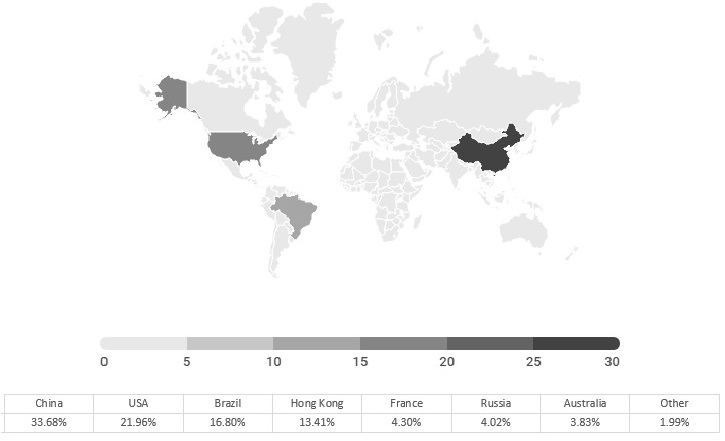
\includegraphics[width=\columnwidth]{section_4/map_countries_memcahced.jpg}
    \caption{Distribution of Memcached \gls{drdos} victims}
    \label{fig:map}
\end{figure}

During the peek period of attack 12 116 unique IP addresses were observed. 8 738 IP addresses received amplified Memcached traffic and were labelled $victim$ as a result. Only 371 of the victim IP addresses received over one Gigabyte per second traffic flows. \textit{Figure~\ref{fig:map}} depicts the global distribution of Memcached \gls{drdos} victims. 4 116 IP addresses were labelled as $port\_scanners$, 881 of which were $memcached\_scanners$. 1 012 IP address had less than 5 flows associated with the Memcached service and were not classified by the network flow sensors.

During the post attack phase only 378 unique IP Addresses were detected by the network flow sensor. Due to the \gls{sanren} servers being patched, no IP addresses were labelled as $victims$ during the post attack phase. This confirms that the software patch did prevent any further \gls{drdos} attacks. 279 IP addresses were found to be performing port scans and 201 were found to be scanning port 11 211 specifically. 191 of the IP addresses labelled as $memcached\_scanners$ did not appear in the list of $memcached\_scanners$ obtained in the pre-attack phase. 29 IP addresses did not produce enough network flow data for classification.

From the post analysis it is clear that the majority of Memcached attack activity has subsided. The analysis also confirmed that the software patches prevented further amplification attacks.


